% !TEX root = ../YourName-Dissertation.tex

\chapter{Questions on the  local level}
This chapter talks about the reaction of subnational governments in the interaction with central government.The most frequently investigated question is the effect of IGT, A bunch of scholars devote time and energy to analyze and evaluate the impact of intergovernmental transfers. I summarize the literature into three categories. The first category focus on the impact on local governments' spending behavior. Under the local governments' spending behavior, two directions are highly documented. First direction concentrate on the effect of intergovernmental transfer on overall spending amounts of subnational government,such as the investigation on flypaper effect. Another direction investigate the micro-segments of the local governments' spending preference. The second category talks about the impact on local governments' revenue collection behavior, such as the investigation on local governments' tax effort, debt expansion tendency and issue and soft budget constrain behavior. The third category is about the effect of intergovernmental transfer across jurisdictions, such as the role of intergovernmental transfer in equalization. This chapter gives an overview on the most innovative literature and introduced the game theory tool under asymmetric setting to generate a theoretical model. The investigation directions can be summarized as Figure \ref*{Figure 3.1}.

\begin{figure}[H]
    \centering
    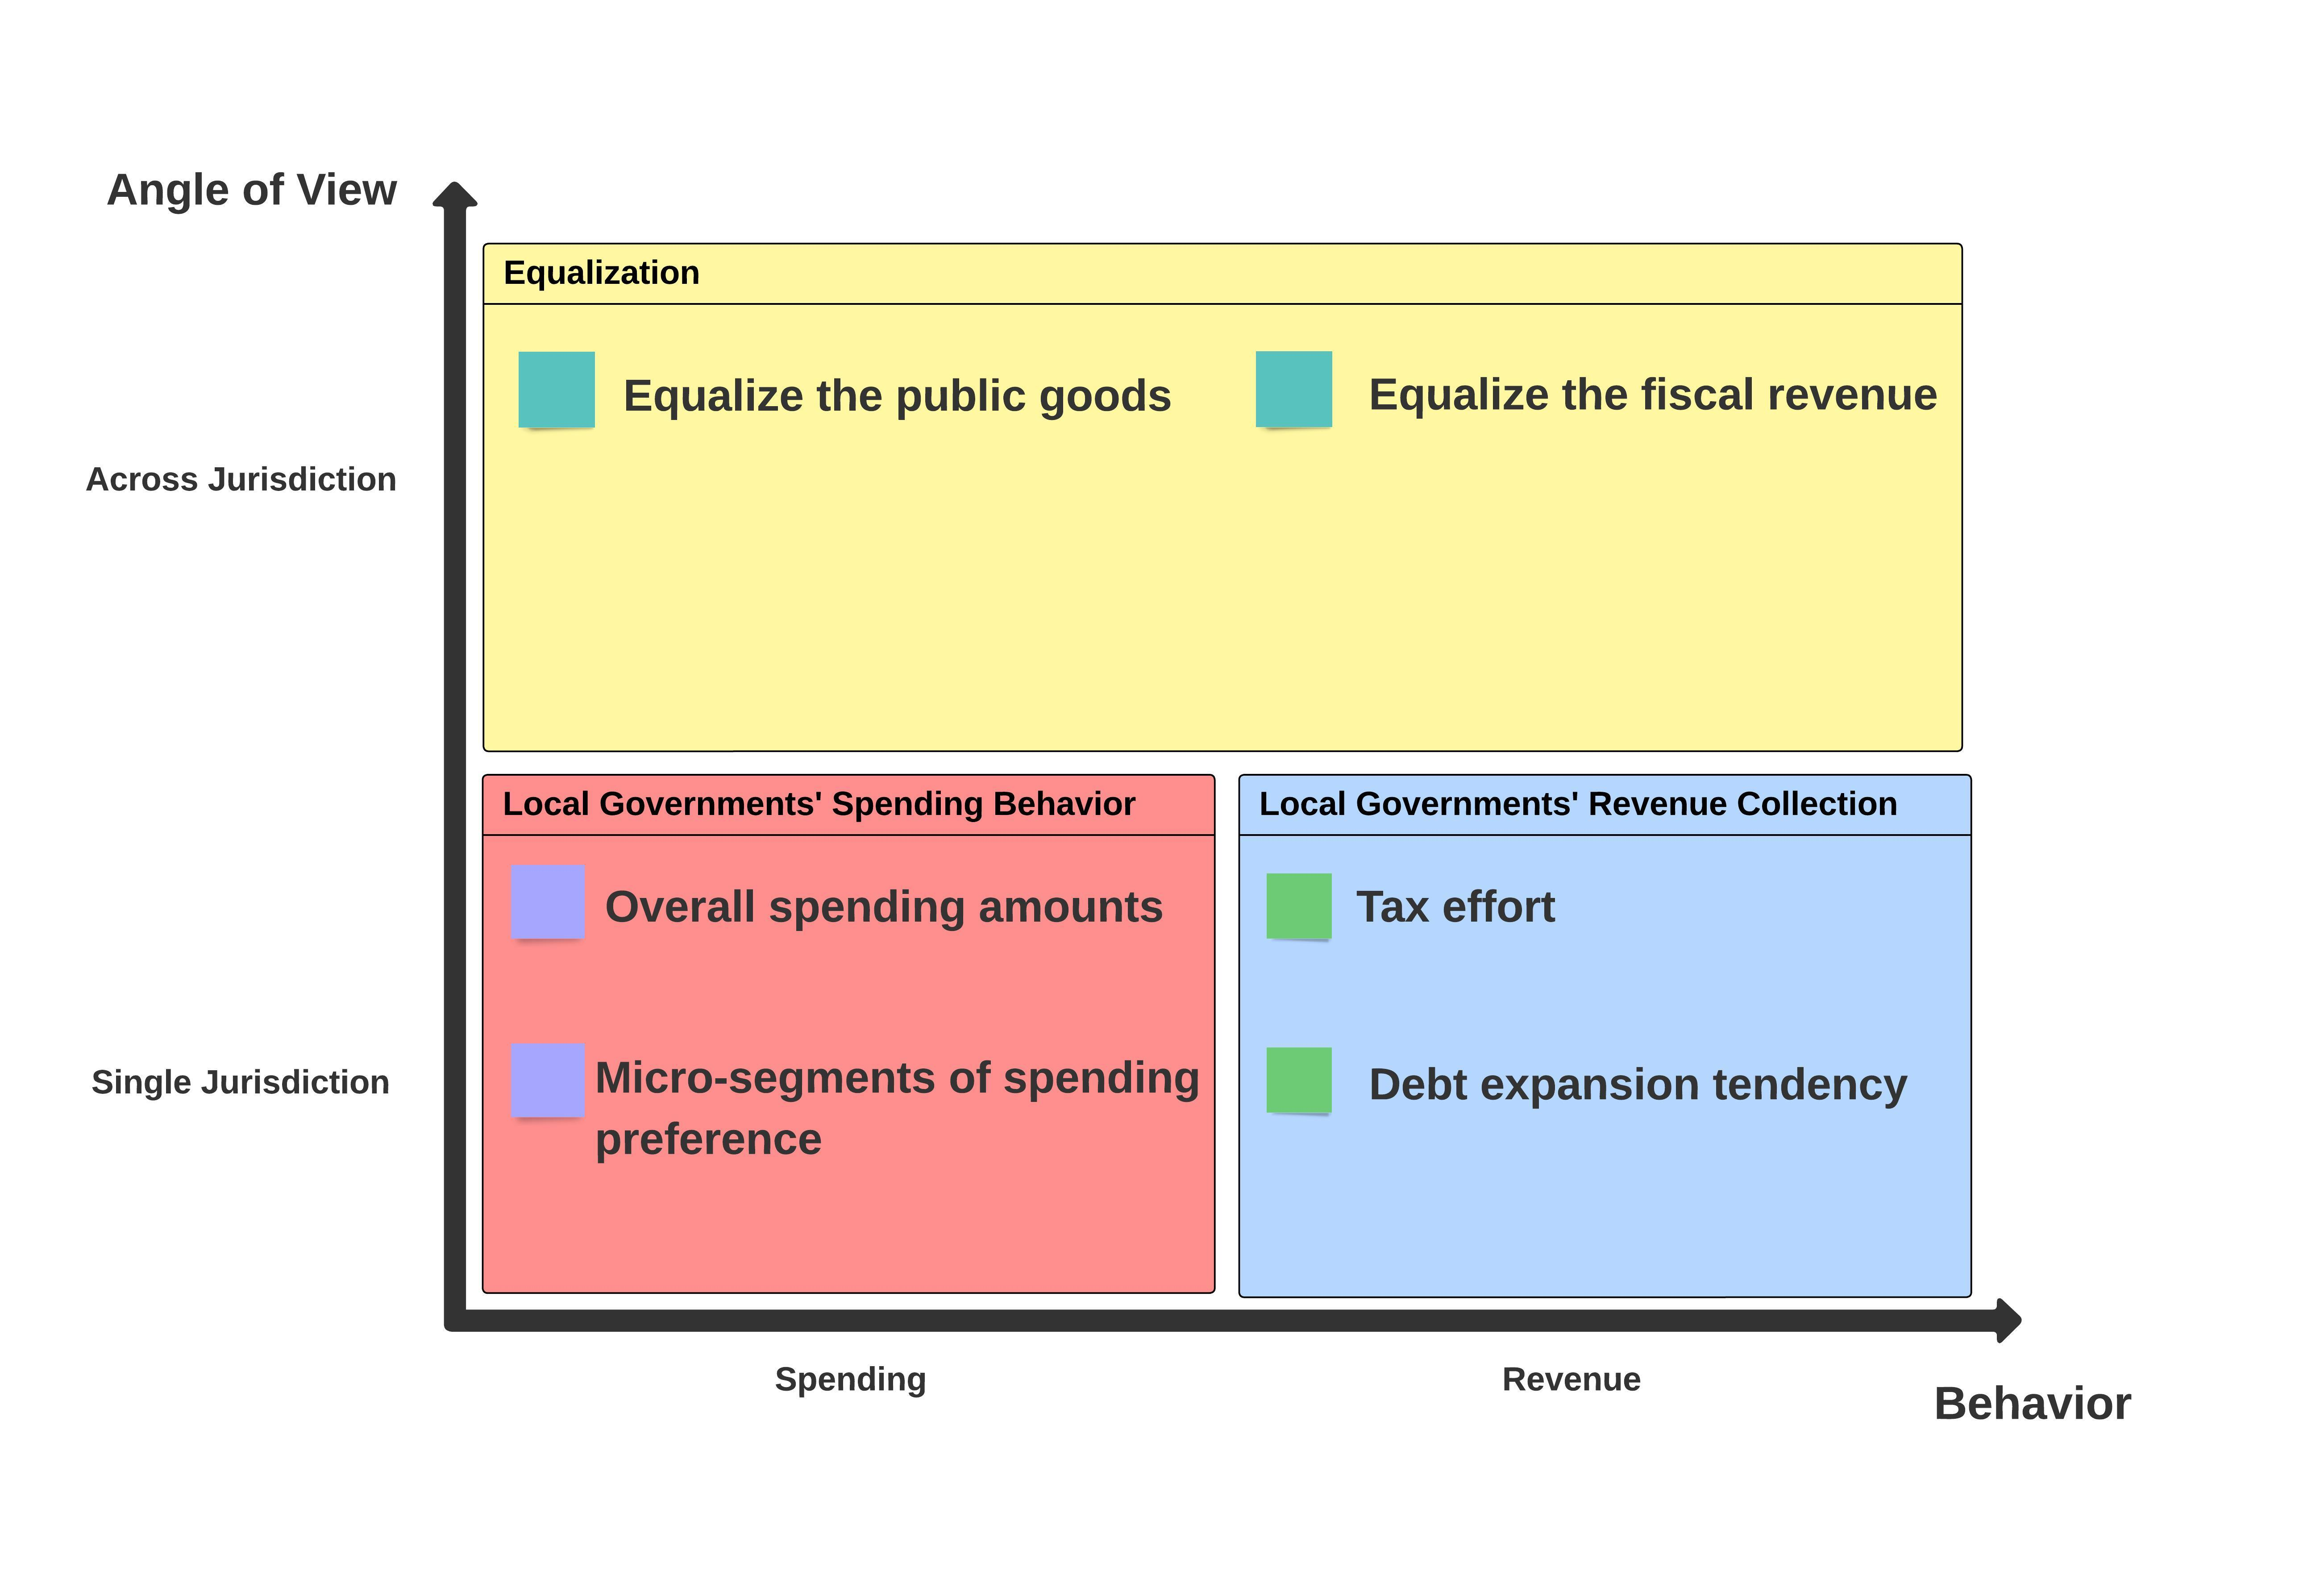
\includegraphics[scale=0.4]{Chapter-3/Figures/Effect of Intergovernmental Transfer.jpeg}
    \caption{Effect of Intergovernmental Transfer
        \texttt{} }
    \label{Figure 3.1}
\end{figure}


\section{Effect of IGT on Local Governments' Spending}

\subsection*{Effect of IGT on Local Governments' Total Spending Amounts}
The most influential phenomenon during the vertical transfer from government in the fiscal federalism literature is the fly paper effect \cite{hines1995anomalies,gamkhar2007impact}. According to Bradford and Oates’s model, a lump sum grant from federal to state or local should be equivalent to the individual revenue increase within the jurisdiction in terms of the effect to stimulate the public expenditure \cite{bradford1971analysis}. The result conclusion is latterly known as equivalence theorem. Two assumptions play fundamental role in equivalence theorem. One is median voter theorem, another one is that federal, state and local government collect tax through lump sum tax. Under this theorem, money is money. However, the empirical evidence doesn’t support this theorem. More specifically, some researchers find that 1 dollar increase in personal increase would increase public expenditure by 0.02 to 0.05 dollar, while 1 dollar increase of intergovernmental transfer would trigger an increase of 0.25 to even 1 dollar in public expenditure \cite{bailey1998flypaper,dollery1996empirical, gamkhar2007impact}. This effect is known as flypaper effect. According to Inman's statistics, over 3,500 research papers investigate the flypaper effect both theoretically and empirically \cite{inman2008flypaper}. In this section, I’m summarizing how scholars in different stages explain the flypaper effect. The understanding of flypaper effect went through a incremental progress chronologically. This progress can be identified as three phrases.

\subsubsection{}




\section{}




